% Created by tikzDevice version 0.7.0 on 2014-09-23 11:36:07
% !TEX encoding = UTF-8 Unicode
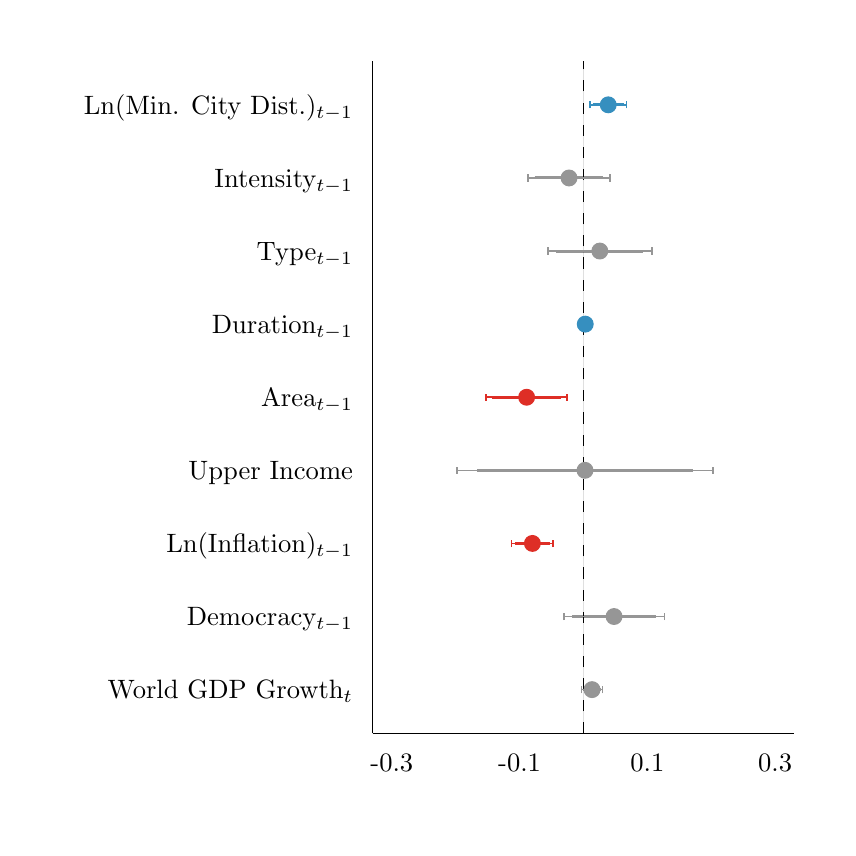
\begin{tikzpicture}[x=1pt,y=1pt]
\definecolor[named]{fillColor}{rgb}{1.00,1.00,1.00}
\path[use as bounding box,fill=fillColor,fill opacity=0.00] (0,0) rectangle (289.08,289.08);
\begin{scope}
\path[clip] (  0.00,  0.00) rectangle (289.08,289.08);
\definecolor[named]{drawColor}{rgb}{1.00,1.00,1.00}
\definecolor[named]{fillColor}{rgb}{1.00,1.00,1.00}

\path[draw=drawColor,line width= 0.6pt,line join=round,line cap=round,fill=fillColor] ( -0.00,  0.00) rectangle (289.08,289.08);
\end{scope}
\begin{scope}
\path[clip] (124.66, 34.03) rectangle (277.03,277.03);
\definecolor[named]{fillColor}{rgb}{1.00,1.00,1.00}

\path[fill=fillColor] (124.66, 34.03) rectangle (277.04,277.03);
\definecolor[named]{drawColor}{rgb}{0.59,0.59,0.59}
\definecolor[named]{fillColor}{rgb}{0.59,0.59,0.59}

\path[draw=drawColor,draw opacity=0.30,line width= 0.3pt,line join=round,fill=fillColor,fill opacity=0.30] (200.10, 49.88) -- (207.76, 49.88);

\path[draw=drawColor,draw opacity=0.30,line width= 0.3pt,line join=round,fill=fillColor,fill opacity=0.30] (193.68, 76.30) -- (230.11, 76.30);
\definecolor[named]{drawColor}{rgb}{0.87,0.18,0.15}
\definecolor[named]{fillColor}{rgb}{0.87,0.18,0.15}

\path[draw=drawColor,draw opacity=0.30,line width= 0.3pt,line join=round,fill=fillColor,fill opacity=0.30] (174.88,102.71) -- (189.88,102.71);
\definecolor[named]{drawColor}{rgb}{0.59,0.59,0.59}
\definecolor[named]{fillColor}{rgb}{0.59,0.59,0.59}

\path[draw=drawColor,draw opacity=0.30,line width= 0.3pt,line join=round,fill=fillColor,fill opacity=0.30] (155.06,129.12) -- (247.73,129.12);
\definecolor[named]{drawColor}{rgb}{0.87,0.18,0.15}
\definecolor[named]{fillColor}{rgb}{0.87,0.18,0.15}

\path[draw=drawColor,draw opacity=0.30,line width= 0.3pt,line join=round,fill=fillColor,fill opacity=0.30] (165.59,155.53) -- (195.00,155.53);
\definecolor[named]{drawColor}{rgb}{0.21,0.56,0.75}
\definecolor[named]{fillColor}{rgb}{0.21,0.56,0.75}

\path[draw=drawColor,draw opacity=0.30,line width= 0.3pt,line join=round,fill=fillColor,fill opacity=0.30] (200.88,181.95) -- (202.07,181.95);
\definecolor[named]{drawColor}{rgb}{0.59,0.59,0.59}
\definecolor[named]{fillColor}{rgb}{0.59,0.59,0.59}

\path[draw=drawColor,draw opacity=0.30,line width= 0.3pt,line join=round,fill=fillColor,fill opacity=0.30] (187.98,208.36) -- (225.50,208.36);

\path[draw=drawColor,draw opacity=0.30,line width= 0.3pt,line join=round,fill=fillColor,fill opacity=0.30] (180.79,234.77) -- (210.45,234.77);
\definecolor[named]{drawColor}{rgb}{0.21,0.56,0.75}
\definecolor[named]{fillColor}{rgb}{0.21,0.56,0.75}

\path[draw=drawColor,draw opacity=0.30,line width= 0.3pt,line join=round,fill=fillColor,fill opacity=0.30] (203.18,261.19) -- (216.39,261.19);
\definecolor[named]{drawColor}{rgb}{0.59,0.59,0.59}
\definecolor[named]{fillColor}{rgb}{0.59,0.59,0.59}

\path[draw=drawColor,line width= 1.1pt,line join=round,fill=fillColor] (200.72, 49.88) -- (207.15, 49.88);

\path[draw=drawColor,line width= 1.1pt,line join=round,fill=fillColor] (196.61, 76.30) -- (227.18, 76.30);
\definecolor[named]{drawColor}{rgb}{0.87,0.18,0.15}
\definecolor[named]{fillColor}{rgb}{0.87,0.18,0.15}

\path[draw=drawColor,line width= 1.1pt,line join=round,fill=fillColor] (176.09,102.71) -- (188.68,102.71);
\definecolor[named]{drawColor}{rgb}{0.59,0.59,0.59}
\definecolor[named]{fillColor}{rgb}{0.59,0.59,0.59}

\path[draw=drawColor,line width= 1.1pt,line join=round,fill=fillColor] (162.51,129.12) -- (240.28,129.12);
\definecolor[named]{drawColor}{rgb}{0.87,0.18,0.15}
\definecolor[named]{fillColor}{rgb}{0.87,0.18,0.15}

\path[draw=drawColor,line width= 1.1pt,line join=round,fill=fillColor] (167.95,155.53) -- (192.63,155.53);
\definecolor[named]{drawColor}{rgb}{0.21,0.56,0.75}
\definecolor[named]{fillColor}{rgb}{0.21,0.56,0.75}

\path[draw=drawColor,line width= 1.1pt,line join=round,fill=fillColor] (200.97,181.95) -- (201.98,181.95);
\definecolor[named]{drawColor}{rgb}{0.59,0.59,0.59}
\definecolor[named]{fillColor}{rgb}{0.59,0.59,0.59}

\path[draw=drawColor,line width= 1.1pt,line join=round,fill=fillColor] (191.00,208.36) -- (222.48,208.36);

\path[draw=drawColor,line width= 1.1pt,line join=round,fill=fillColor] (183.17,234.77) -- (208.07,234.77);
\definecolor[named]{drawColor}{rgb}{0.21,0.56,0.75}
\definecolor[named]{fillColor}{rgb}{0.21,0.56,0.75}

\path[draw=drawColor,line width= 1.1pt,line join=round,fill=fillColor] (204.24,261.19) -- (215.33,261.19);
\definecolor[named]{drawColor}{rgb}{0.00,0.00,0.00}
\definecolor[named]{fillColor}{rgb}{0.00,0.00,0.00}

\path[draw=drawColor,line width= 0.6pt,dash pattern=on 4pt off 4pt ,line join=round,fill=fillColor] (200.85, 34.03) -- (200.85,277.03);
\definecolor[named]{drawColor}{rgb}{0.21,0.56,0.75}
\definecolor[named]{fillColor}{rgb}{0.21,0.56,0.75}

\path[draw=drawColor,line width= 0.4pt,line join=round,line cap=round,fill=fillColor] (209.79,261.19) circle (  2.85);
\definecolor[named]{drawColor}{rgb}{0.59,0.59,0.59}
\definecolor[named]{fillColor}{rgb}{0.59,0.59,0.59}

\path[draw=drawColor,line width= 0.4pt,line join=round,line cap=round,fill=fillColor] (195.62,234.77) circle (  2.85);

\path[draw=drawColor,line width= 0.4pt,line join=round,line cap=round,fill=fillColor] (206.74,208.36) circle (  2.85);
\definecolor[named]{drawColor}{rgb}{0.21,0.56,0.75}
\definecolor[named]{fillColor}{rgb}{0.21,0.56,0.75}

\path[draw=drawColor,line width= 0.4pt,line join=round,line cap=round,fill=fillColor] (201.47,181.95) circle (  2.85);
\definecolor[named]{drawColor}{rgb}{0.87,0.18,0.15}
\definecolor[named]{fillColor}{rgb}{0.87,0.18,0.15}

\path[draw=drawColor,line width= 0.4pt,line join=round,line cap=round,fill=fillColor] (180.29,155.53) circle (  2.85);
\definecolor[named]{drawColor}{rgb}{0.59,0.59,0.59}
\definecolor[named]{fillColor}{rgb}{0.59,0.59,0.59}

\path[draw=drawColor,line width= 0.4pt,line join=round,line cap=round,fill=fillColor] (201.39,129.12) circle (  2.85);
\definecolor[named]{drawColor}{rgb}{0.87,0.18,0.15}
\definecolor[named]{fillColor}{rgb}{0.87,0.18,0.15}

\path[draw=drawColor,line width= 0.4pt,line join=round,line cap=round,fill=fillColor] (182.38,102.71) circle (  2.85);
\definecolor[named]{drawColor}{rgb}{0.59,0.59,0.59}
\definecolor[named]{fillColor}{rgb}{0.59,0.59,0.59}

\path[draw=drawColor,line width= 0.4pt,line join=round,line cap=round,fill=fillColor] (211.89, 76.30) circle (  2.85);

\path[draw=drawColor,line width= 0.4pt,line join=round,line cap=round,fill=fillColor] (203.93, 49.88) circle (  2.85);

\path[draw=drawColor,line width= 0.6pt,line join=round] (207.76, 48.56) --
	(207.76, 51.20);

\path[draw=drawColor,line width= 0.6pt,line join=round] (207.76, 49.88) --
	(200.10, 49.88);

\path[draw=drawColor,line width= 0.6pt,line join=round] (200.10, 48.56) --
	(200.10, 51.20);

\path[draw=drawColor,line width= 0.6pt,line join=round] (230.11, 74.97) --
	(230.11, 77.62);

\path[draw=drawColor,line width= 0.6pt,line join=round] (230.11, 76.30) --
	(193.68, 76.30);

\path[draw=drawColor,line width= 0.6pt,line join=round] (193.68, 74.97) --
	(193.68, 77.62);
\definecolor[named]{drawColor}{rgb}{0.87,0.18,0.15}

\path[draw=drawColor,line width= 0.6pt,line join=round] (189.88,101.39) --
	(189.88,104.03);

\path[draw=drawColor,line width= 0.6pt,line join=round] (189.88,102.71) --
	(174.88,102.71);

\path[draw=drawColor,line width= 0.6pt,line join=round] (174.88,101.39) --
	(174.88,104.03);
\definecolor[named]{drawColor}{rgb}{0.59,0.59,0.59}

\path[draw=drawColor,line width= 0.6pt,line join=round] (247.73,127.80) --
	(247.73,130.44);

\path[draw=drawColor,line width= 0.6pt,line join=round] (247.73,129.12) --
	(155.06,129.12);

\path[draw=drawColor,line width= 0.6pt,line join=round] (155.06,127.80) --
	(155.06,130.44);
\definecolor[named]{drawColor}{rgb}{0.87,0.18,0.15}

\path[draw=drawColor,line width= 0.6pt,line join=round] (195.00,154.21) --
	(195.00,156.86);

\path[draw=drawColor,line width= 0.6pt,line join=round] (195.00,155.53) --
	(165.59,155.53);

\path[draw=drawColor,line width= 0.6pt,line join=round] (165.59,154.21) --
	(165.59,156.86);
\definecolor[named]{drawColor}{rgb}{0.21,0.56,0.75}

\path[draw=drawColor,line width= 0.6pt,line join=round] (202.07,180.63) --
	(202.07,183.27);

\path[draw=drawColor,line width= 0.6pt,line join=round] (202.07,181.95) --
	(200.88,181.95);

\path[draw=drawColor,line width= 0.6pt,line join=round] (200.88,180.63) --
	(200.88,183.27);
\definecolor[named]{drawColor}{rgb}{0.59,0.59,0.59}

\path[draw=drawColor,line width= 0.6pt,line join=round] (225.50,207.04) --
	(225.50,209.68);

\path[draw=drawColor,line width= 0.6pt,line join=round] (225.50,208.36) --
	(187.98,208.36);

\path[draw=drawColor,line width= 0.6pt,line join=round] (187.98,207.04) --
	(187.98,209.68);

\path[draw=drawColor,line width= 0.6pt,line join=round] (210.45,233.45) --
	(210.45,236.09);

\path[draw=drawColor,line width= 0.6pt,line join=round] (210.45,234.77) --
	(180.79,234.77);

\path[draw=drawColor,line width= 0.6pt,line join=round] (180.79,233.45) --
	(180.79,236.09);
\definecolor[named]{drawColor}{rgb}{0.21,0.56,0.75}

\path[draw=drawColor,line width= 0.6pt,line join=round] (216.39,259.87) --
	(216.39,262.51);

\path[draw=drawColor,line width= 0.6pt,line join=round] (216.39,261.19) --
	(203.18,261.19);

\path[draw=drawColor,line width= 0.6pt,line join=round] (203.18,259.87) --
	(203.18,262.51);
\end{scope}
\begin{scope}
\path[clip] (  0.00,  0.00) rectangle (289.08,289.08);
\definecolor[named]{drawColor}{rgb}{0.00,0.00,0.00}

\path[draw=drawColor,line width= 0.6pt,line join=round] (124.66, 34.03) --
	(124.66,277.03);
\end{scope}
\begin{scope}
\path[clip] (  0.00,  0.00) rectangle (289.08,289.08);
\definecolor[named]{drawColor}{rgb}{0.00,0.00,0.00}

\node[text=drawColor,anchor=base east,inner sep=0pt, outer sep=0pt, scale=  0.96] at (117.55, 46.58) {World GDP Growth$_{t}$};

\node[text=drawColor,anchor=base east,inner sep=0pt, outer sep=0pt, scale=  0.96] at (117.55, 72.99) {Democracy$_{t-1}$};

\node[text=drawColor,anchor=base east,inner sep=0pt, outer sep=0pt, scale=  0.96] at (117.55, 99.40) {Ln(Inflation)$_{t-1}$};

\node[text=drawColor,anchor=base east,inner sep=0pt, outer sep=0pt, scale=  0.96] at (117.55,125.82) {Upper Income};

\node[text=drawColor,anchor=base east,inner sep=0pt, outer sep=0pt, scale=  0.96] at (117.55,152.23) {Area$_{t-1}$};

\node[text=drawColor,anchor=base east,inner sep=0pt, outer sep=0pt, scale=  0.96] at (117.55,178.64) {Duration$_{t-1}$};

\node[text=drawColor,anchor=base east,inner sep=0pt, outer sep=0pt, scale=  0.96] at (117.55,205.06) {Type$_{t-1}$};

\node[text=drawColor,anchor=base east,inner sep=0pt, outer sep=0pt, scale=  0.96] at (117.55,231.47) {Intensity$_{t-1}$};

\node[text=drawColor,anchor=base east,inner sep=0pt, outer sep=0pt, scale=  0.96] at (117.55,257.88) {Ln(Min. City Dist.)$_{t-1}$};
\end{scope}
\begin{scope}
\path[clip] (  0.00,  0.00) rectangle (289.08,289.08);
\definecolor[named]{drawColor}{rgb}{0.00,0.00,0.00}

\path[draw=drawColor,line width= 0.6pt,line join=round] (124.66, 34.03) --
	(277.03, 34.03);
\end{scope}
\begin{scope}
\path[clip] (  0.00,  0.00) rectangle (289.08,289.08);
\definecolor[named]{drawColor}{rgb}{0.00,0.00,0.00}

\node[text=drawColor,anchor=base,inner sep=0pt, outer sep=0pt, scale=  0.96] at (131.59, 20.31) {-0.3};

\node[text=drawColor,anchor=base,inner sep=0pt, outer sep=0pt, scale=  0.96] at (177.76, 20.31) {-0.1};

\node[text=drawColor,anchor=base,inner sep=0pt, outer sep=0pt, scale=  0.96] at (223.94, 20.31) {0.1};

\node[text=drawColor,anchor=base,inner sep=0pt, outer sep=0pt, scale=  0.96] at (270.11, 20.31) {0.3};
\end{scope}
\end{tikzpicture}
